\documentclass[a4paper, 11pt]{article} % Font size (can be 10pt, 11pt or 12pt) and paper size (remove a4paper for US letter paper)

\usepackage[protrusion=true,expansion=true]{microtype} % Better typography
\usepackage{graphicx} % Required for including pictures
\usepackage{wrapfig} % Allows in-line images

\usepackage{mathpazo} % Use the Palatino font
\usepackage[T1]{fontenc} % Required for accented characters
\linespread{1.05} % Change line spacing here, Palatino benefits from a slight increase by default

\makeatletter
\renewcommand\@biblabel[1]{\textbf{#1.}} % Change the square brackets for each bibliography item from '[1]' to '1.'
\renewcommand{\@listI}{\itemsep=0pt} % Reduce the space between items in the itemize and enumerate environments and the bibliography

\renewcommand{\maketitle}{ % Customize the title - do not edit title and author name here, see the TITLE block below
\begin{flushright} % Right align
{\LARGE\@title} % Increase the font size of the title

\vspace{50pt} % Some vertical space between the title and author name

{\large\@author} % Author name
\\\@date % Date

\vspace{40pt} % Some vertical space between the author block and abstract
\end{flushright}
}

%----------------------------------------------------------------------------------------
%	TITLE
%----------------------------------------------------------------------------------------

\title{\textbf{Transistors}\\ % Title
Quick introduction} % Subtitle

\author{\textsc{David Alejandro Trejo Pizzo} % Author
\\{\textit{Universidad de Palermo}}} % Institution

\date{\today} % Date

%----------------------------------------------------------------------------------------

\begin{document}

\maketitle % Print the title section

%----------------------------------------------------------------------------------------
%	ABSTRACT AND KEYWORDS
%----------------------------------------------------------------------------------------

%\renewcommand{\abstractname}{Summary} % Uncomment to change the name of the abstract to something else

\begin{abstract}
This document intends to give a quick introduction to transistors, polarization, amplifiers and some particular applications of operational amplifiers.
\end{abstract}

\hspace*{3,6mm}\textit{Keywords:} transistor , amplifiers , gates% Keywords

\vspace{30pt} % Some vertical space between the abstract and first section

%----------------------------------------------------------------------------------------
%	ESSAY BODY
%----------------------------------------------------------------------------------------

\section*{Introduction}

Transistors make our electronics world go around. They are critical as a control source in just about every modern circuit. Sometimes you see them, but more-often-than-not they are hidden deep within the die of an integrated circuit. In this tutorial we will introduce you to the basics of the most common transistor around: the bi-polar junction transistor (BJT).

\begin{center}
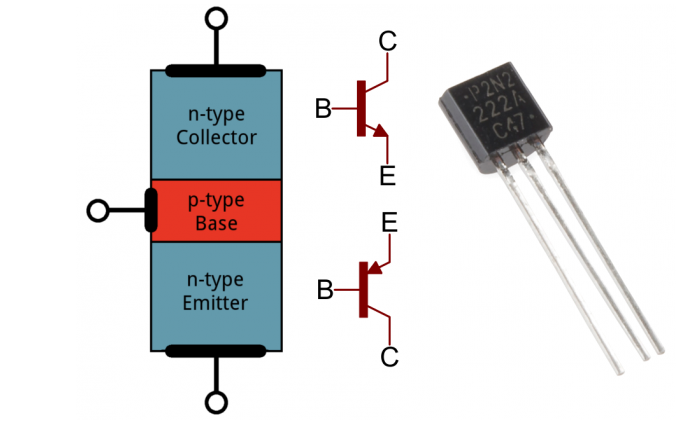
\includegraphics[width=300pt]{tran1}
\end{center}

In small, discrete quantities, transistors can be used to create simple electronic switches, digital logic, and signal amplifying circuits. In quantities of thousands, millions, and even billions, transistors are interconnected and embedded into tiny chips to create computer memories, microprocessors, and other complex ICs.

\section*{Symbols, Pins, and Construction}

Transistors are fundamentally three-terminal devices. On a bipolar junction transistor (BJT), those pins are labeled collector (C), base (B), and emitter (E). The circuit symbols for both the NPN and PNP BJT are below:

\begin{center}
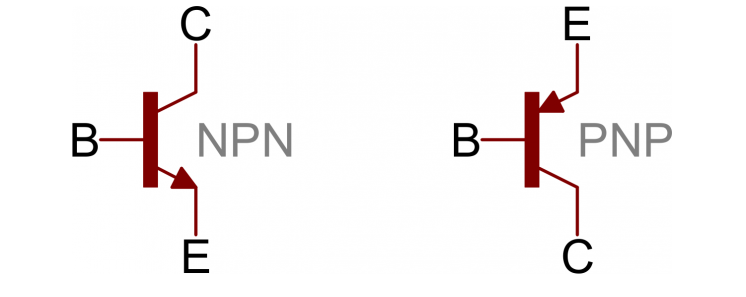
\includegraphics[width=300pt]{tran2}
\end{center}

The only difference between an NPN and PNP is the direction of the arrow on the emitter. The arrow on an NPN points out, and on the PNP it points in. A useful mnemonic for remembering which is which is:

\begin{center}
\textbf{NPN: Not pointing in}
\end{center}

Backwards logic, but it works!

\subsection*{Transistor construction}

Transistors rely on semiconductors to work their magic. A semiconductor is a material that is not quite a pure conductor (like copper wire) but also not an insulator (like air). The conductivity of a semiconductor - how easily it allows electrons to flow - depends on variables like temperature or the presence of more or less electrons. Let's look briefly under the hood of a transistor. Do not worry, we won't dig too deeply into quantum physics.

\subsubsection*{A Transistor as Two Diodes}

Transistors are kind of like an extension of another semiconductor component: diodes. In a way transistors are just two diodes with their cathodes (or anodes) tied together:

\begin{center}
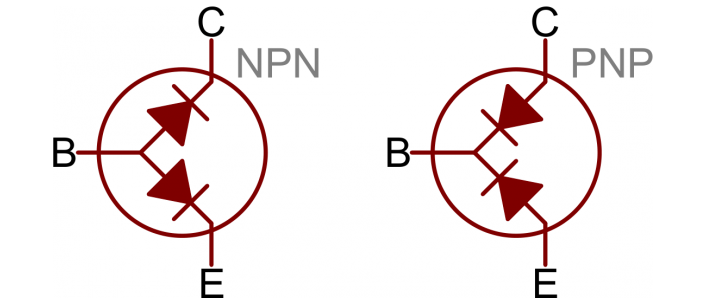
\includegraphics[width=300pt]{tran3}
\end{center}

The diode connecting base to emitter is the important one here; it matches the direction of the arrow on the schematic symbol, and shows you which way current is intended to flow through the transistor.\\

The diode representation is a good place to start, but it is far from accurate. Do not base your understanding of a transistor's operation on that model (and definitely do not try to replicate it on a breadboard, it won't work). There is a whole lot of weird quantum physics level stuff controlling the interactions between the three terminals.\\

(This model is useful if you need to test a transistor. Using the diode (or resistance) test function on a multimeter, you can measure across the BE and BC terminals to check for the presence of those "diodes".)

\subsubsection*{Transistor Structure and Operation}

Transistors are built by stacking three different layers of semiconductor material together. Some of those layers have extra electrons added to them (a process called "doping"), and others have electrons removed (doped with "holes" - the absence of electrons). A semiconductor material with extra electrons is called an \textbf{n-type} (\textbf{n} for negative because electrons have a negative charge) and a material with electrons removed is called a \textbf{p-type} (for positive).

\begin{center}
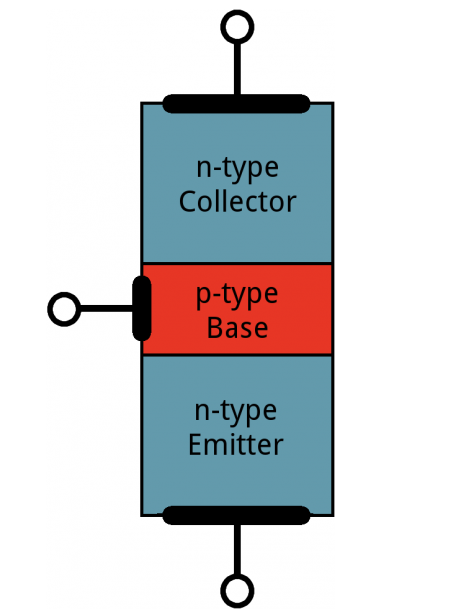
\includegraphics[width=300pt]{tran4}
\end{center}

With some hand waving, we can say electrons can easily flow from n regions to p regions, as long as they have a little force (voltage) to push them. But flowing from a p region to an n region is really hard (requires a lot of voltage). But the special thing about a transistor - the part that makes our two-diode model obsolete - is the fact that electrons can easily flow from the p-type base to the n-type collector as long as the base-emitter junction is forward biased (meaning the base is at a higher voltage than the emitter).

\begin{center}
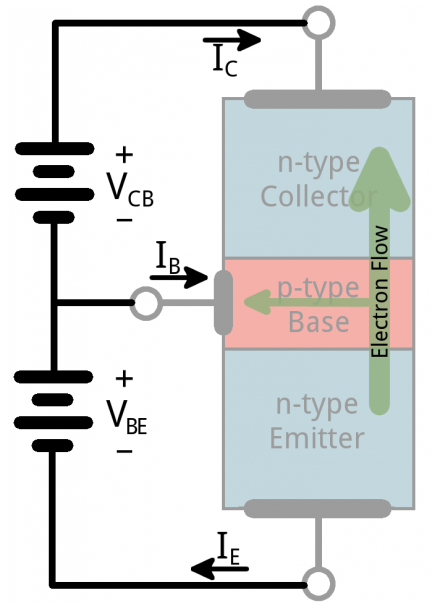
\includegraphics[width=300pt]{tran5}
\end{center}

The NPN transistor is designed to pass electrons from the emitter to the collector (so conventional current flows from collector to emitter). The emitter "emits" electrons into the base, which controls the number of electrons the emitter emits. Most of the electrons emitted are "collected" by the collector, which sends them along to the next part of the circuit.\\

A PNP works in a same but opposite fashion. The base still controls current flow, but that current flows in the opposite direction - from emitter to collector. Instead of electrons, the emitter emits "holes" (a conceptual absence of electrons) which are collected by the collector.\\

The transistor is kind of like an electron valve. The base pin is like a handle you might adjust to allow more or less electrons to flow from emitter to collector. Let's investigate this analogy further...

\section*{Extending the Water Analogy}

If you have been reading a lot of electricity concept tutorials lately, you are probably used to water analogies. We say that current is analogous to the flow rate of water, voltage is the pressure pushing that water through a pipe, and resistance is the width of the pipe.

\begin{center}
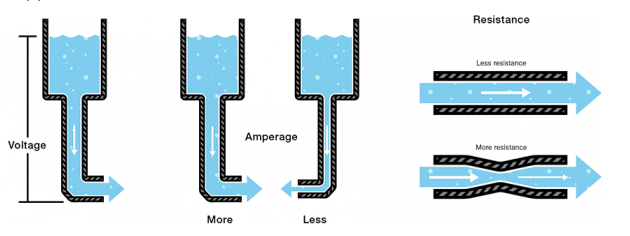
\includegraphics[width=300pt]{tran6}
\end{center}

Unsurprisingly, the water analogy can be extended to transistors as well: a transistor is like a water valve - a mechanism we can use to control the flow rate.\\

There are three states we can use a valve in, each of which has a different effect on the flow rate in a system.\\

\textbf{1) On - Short Circuit}\\

A valve can be completely opened, allowing water to flow freely - passing through as if the valve was not even present.

\begin{center}
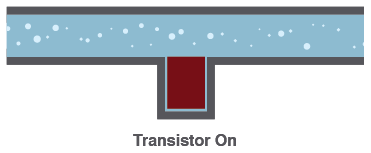
\includegraphics[width=300pt]{tran7}
\end{center}

Likewise, under the right circumstances, a transistor can look like a short circuit between the collector and emitter pins. Current is free to flow through the collector, and out the emitter.\\

\textbf{2) Off - Open Circuit}

When it is closed, a valve can completely stop the flow of water.

\begin{center}
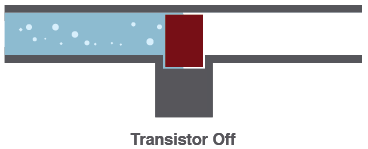
\includegraphics[width=300pt]{tran8}
\end{center}

In the same way, a transistor can be used to create an open circuit between the collector and emitter pins.

\textbf{3) Linear Flow Control}

With some precise tuning, a valve can be adjusted to finely control the flow rate to some point between fully open and closed.

\begin{center}
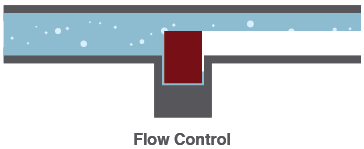
\includegraphics[width=300pt]{tran9}
\end{center}

A transistor can do the same thing – linearly controlling the current through a circuit at some point between fully off (an open circuit) and fully on (a short circuit).\\

From our water analogy, the width of a pipe is similar to the resistance in a circuit. If a valve can finely adjust the width of a pipe, then a transistor can finely adjust the resistance between collector and emitter. So, in a way, a transistor is like a variable, adjustable resistor.

\subsection*{Amplifying Power}

There is another analogy we can wrench into this. Imagine if, with the slight turn of a valve, you could control the flow rate of the Hoover Dam's flow gates. The measly amount of force you might put into twisting that knob has the potential to create a force thousands of times stronger. We are stretching the analogy to its limits, but this idea carries over to transistors too. Transistors are special because they can amplify electrical signals, turning a low-power signal into a similar signal of much higher power.\\

Kind of. There is a lot more to it, but that is a good place to start! Check out the next section for a more detailed explanation of the operation of a transistor.

\section*{Operation Modes}

Unlike resistors, which enforce a linear relationship between voltage and current, transistors are non-linear devices. They have four distinct modes of operation, which describe the current flowing through them. (When we talk about current flow through a transistor, we usually mean current flowing from collector to emitter of an NPN.)

The four transistor operation modes are:

\begin{itemize}
\item Saturation - The transistor acts like a short circuit. Current freely flows from collector to emitter.
\item Cut-off - The transistor acts like an open circuit. No current flows from collector to emitter.
\item Active - The current from collector to emitter is proportional to the current flowing into the base.
\item Reverse-Active - Like active mode, the current is proportional to the base current, but it flows in reverse. Current flows from emitter to collector (not, exactly, the purpose transistors were designed for).
\end{itemize}

To determine which mode a transistor is in, we need to look at the voltages on each of the three pins, and how they relate to each other. The voltages from base to emitter (VBE), and the from base to collector (VBC) set the transistor's mode:

\begin{center}
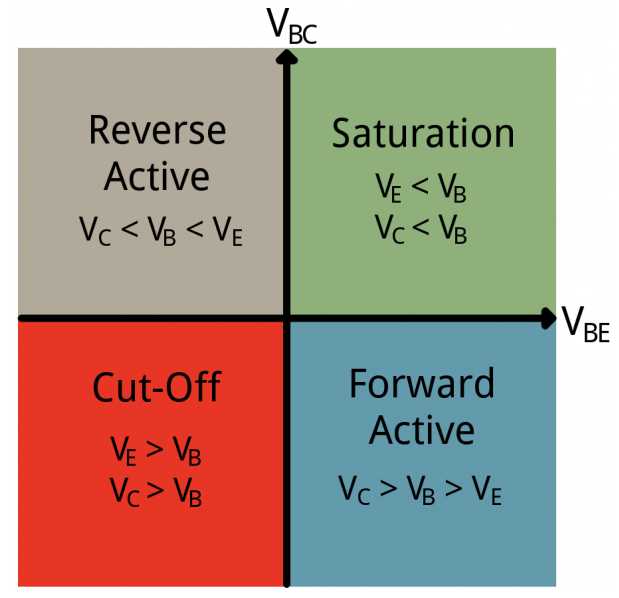
\includegraphics[width=300pt]{tran10}
\end{center}

The simplified quadrant graph above shows how positive and negative voltages at those terminals affect the mode. In reality it is a bit more complicated than that.\\

Let's look at all four transistor modes individually; we will investigate how to put the device into that mode, and what effect it has on current flow.\\

Note: The majority of this page focuses on NPN transistors. To understand how a PNP transistor works, simply flip the polarity or > and < signs.\\

\subsection*{Saturation Mode}

Saturation is the on mode of a transistor. A transistor in saturation mode acts like a short circuit between collector and emitter.

\begin{center}
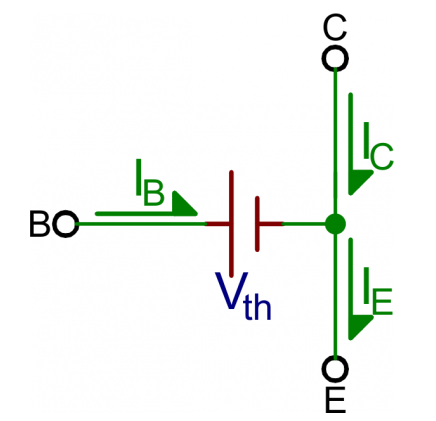
\includegraphics[width=200pt]{tran11}
\end{center}

In saturation mode both of the "diodes" in the transistor are forward biased. That means $VBE$ must be greater than 0, and so must $VBC$. In other words, $VB$ must be higher than both $VE$ and $VC$.

$$V_{B} > V_{C}$$

$$V_{B} > V_{E}$$

Because the junction from base to emitter looks just like a diode, in reality, $VBE$ must be greater than a threshold voltage to enter saturation. There are many abbreviations for this voltage drop - $V_{th}$, $V_{\lambda}$, and $V_{d}$ are a few - and the actual value varies between transistors (and even further by temperature). For a lot of transistors (at room temperature) we can estimate this drop to be about $0.6V$.\\

Another reality bummer: there won't be perfect conduction between emitter and collector. A small voltage drop will form between those nodes. Transistor datasheets will define this voltage as $CE$ saturation voltage $VCE(sat)$ - a voltage from collector to emitter required for saturation. This value is usually around $0.05-0.2V$. This value means that $VC$ must be slightly greater than $VE$ (but both still less than $VB$) to get the transistor in saturation mode.

\subsection*{Cutoff Mode}

Cutoff mode is the opposite of saturation. A transistor in cutoff mode is off - there is no collector current, and therefore no emitter current. It almost looks like an open circuit.

\begin{center}
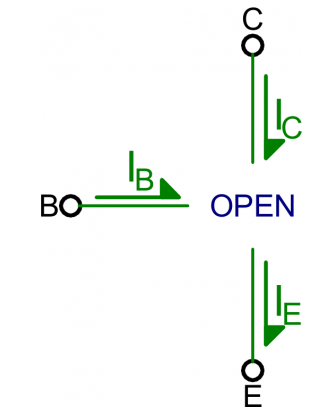
\includegraphics[width=200pt]{tran12}
\end{center}

To get a transistor into cutoff mode, the base voltage must be less than both the emitter and collector voltages. $VBC$ and $VBE$ must both be negative.

$$V_{C} > V_{B}$$

$$V_{E} > V_{B}$$

In reality, $VBE$ can be anywhere between 0V and Vth $(\approx 0.6V)$ to achieve cutoff mode.

\subsection*{Active Mode}

To operate in active mode, a transistor's $V_{BE}$ must be greater than zero and $V_{BC}$ must be negative. Thus, the base voltage must be less than the collector, but greater than the emitter. That also means the collector must be greater than the emitter.

$$V_{C} > V_{B} > V_{E}$$

In reality, we need a non-zero forward voltage drop (abbreviated either $V_{th}$, $V_{\lambda}$, or $V_{d}$) from base to emitter ($V_{BE}$) to "turn on" the transistor. Usually this voltage is usually around $0.6V$.

\subsection*{Amplifying in Active Mode}

Active mode is the most powerful mode of the transistor because it turns the device into an amplifier. Current going into the base pin amplifies current going into the collector and out the emitter.\\

Our shorthand notation for the gain (amplification factor) of a transistor is $\beta$ (you may also see it as $\beta_{F}$, or $h_{FE}$). $\beta$ linearly relates the collector current ($I_{C}$) to the base current ($I_{B}$):

$$I_{C} = \beta I_{B}$$

The actual value of $\beta$ varies by transistor. It is usually around 100, but can range from 50 to 200... even 2000, depending on which transistor you are using and how much current is running through it. If your transistor had a $\beta$ of 100, for example, that'd mean an input current of 1mA into the base could produce $100mA$ current through the collector.

\begin{center}
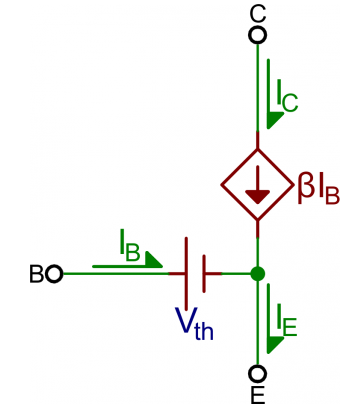
\includegraphics[width=200pt]{tran13}
\end{center}

What about the emitter current, $I_{E}?$ In active mode, the collector and base currents go into the device, and the IE comes out. To relate the emitter current to collector current, we have another constant value: $\alpha$ (is the common-base current gain), it relates those currents as such:

$$I_{C} = \alpha I_{E}$$

$\alpha$ is usually very close to, but less than, 1. That means $I_{C}$ is very close to, but less than $I_{E}$ in active mode. You can use $\beta$ to calculate $\alpha$, or vice-versa:

$$ \beta = \frac{\alpha}{1-\alpha}$$

$$ \alpha = \frac{\beta}{\beta +1}$$

If $\beta$ is 100, for example, that means $\alpha$ is 0.99. So, if $I_{C}$ is 100mA, for example, then $I_{E}$ is 101mA.

\subsection*{Reverse Active}

Just as saturation is the opposite of cutoff, reverse active mode is the opposite of active mode. A transistor in reverse active mode conducts, even amplifies, but current flows in the opposite direction, from emitter to collector. The downside to reverse active mode is the $\beta$ ($\beta$R in this case) is much smaller.\\

To put a transistor in reverse active mode, the emitter voltage must be greater than the base, which must be greater than the collector ($V_{BE}<0$ and $V_{BC}>0$).

$$ V_{C} < V_{B} < V_{E}$$

Reverse active mode is not usually a state in which you want to drive a transistor. It is good to know it is there, but it is rarely designed into an application.

\subsection*{Relating to the PNP}

After everything we have talked about on this page, we have still only covered half of the BJT spectrum. What about PNP transistors? PNP's work a lot like the NPN's - they have the same four modes - but everything is turned around. To find out which mode a PNP transistor is in, reverse all of the < and > signs.\\

For example, to put a PNP into saturation $V_{C}$ and $V_{E}$ must be higher than $V_{B}$. You pull the base low to turn the PNP on, and make it higher than the collector and emitter to turn it off. And, to put a PNP into active mode, $V_{E}$ must be at a higher voltage than $V_{B}$, which must be higher than $V_{C}$.\\

In summary:\\


\begin{center}
\begin{tabular}{|c|c|c|}
\hline 
\textbf{Voltage relations} & \textbf{NPN mode} & \textbf{PNP mode} \\ 
\hline 
$V_{E} < V_{B} < V_{C}$ & Active & Reverse \\ 
\hline 
$V_{E} < V_{B} > V_{C}$ & Saturation & Cutoff \\ 
\hline 
$V_{E} > V_{B} < V_{C}$  & Cutoff & Saturation \\ 
\hline 
$V_{E} > V_{B} > V_{C}$  & Reverse & Active \\ 
\hline 
\end{tabular} 
\end{center}

Another opposing characteristic of the NPNs and PNPs is the direction of current flow. In active and saturation modes, \textbf{current in a PNP flows from emitter to collector}. This means the emitter must generally be at a higher voltage than the collector.\\

If you are burnt out on conceptual stuff, take a trip to the next section. The best way to learn how a transistor works is to examine it in real-life circuits. Let's look at some applications!

\section*{Applications I: Switches}

One of the most fundamental applications of a transistor is using it to control the flow of power to another part of the circuit - using it as an electric switch. Driving it in either cutoff or saturation mode, the transistor can create the binary on/off effect of a switch.??

Transistor switches are critical circuit-building blocks; they are used to make logic gates, which go on to create microcontrollers, microprocessors, and other integrated circuits. Below are a few example circuits.

\subsection*{Transistor Switch}

Let's look at the most fundamental transistor-switch circuit: an NPN switch. Here we use an NPN to control a high-power LED:

\begin{center}
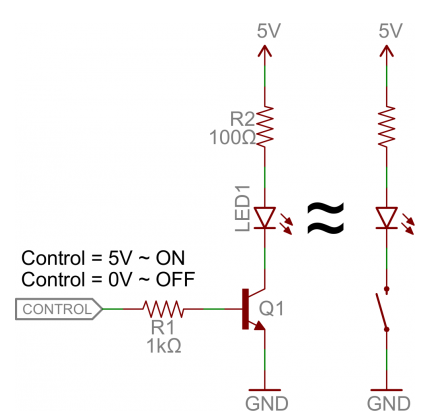
\includegraphics[width=300pt]{tran14}
\end{center}

Our control input flows into the base, the output is tied to the collector, and the emitter is kept at a fixed voltage.\\

While a normal switch would require an actuator to be physically flipped, this switch is controlled by the voltage at the base pin. A microcontroller I/O pin, like those on an Arduino, can be programmed to go high or low to turn the LED on or off.\\

When the voltage at the base is greater than 0.6V (or whatever your transistor's Vth might be), the transistor starts saturating and looks like a short circuit between collector and emitter. When the voltage at the base is less than 0.6V the transistor is in cutoff mode - no current flows because it looks like an open circuit between $C$ and $E$.\\

The circuit above is called a low-side switch, because the switch - our transistor - is on the low (ground) side of the circuit. Alternatively, we can use a PNP transistor to create a high-side switch:

\begin{center}
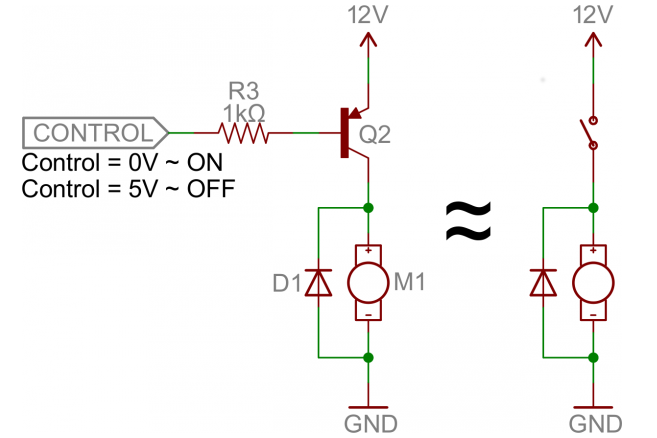
\includegraphics[width=300pt]{tran15}
\end{center}

Similar to the NPN circuit, the base is our input, and the emitter is tied to a constant voltage. This time however, the emitter is tied high, and the load is connected to the transistor on the ground side.\\

This circuit works just as well as the NPN-based switch, but there is one huge difference: to turn the load "on" the base must be low. This can cause complications, especially if the load's high voltage ($V_{CC}$ in this picture) is higher than our control input's high voltage. For example, this circuit wouldn't work if you were trying to use a 5V-operating Arduino to switch on a 12V motor. In that case it'd be impossible to turn the switch off because VB would always be less than VE.

\subsection*{Base Resistors!}

You will notice that each of those circuits uses a series resistor between the control input and the base of the transistor. Do not forget to add this resistor! A transistor without a resistor on the base is like an LED with no current-limiting resistor.\\

Recall that, in a way, a transistor is just a pair of interconnected diodes. We are forward-biasing the base-emitter diode to turn the load on. The diode only needs 0.6V to turn on, more voltage than that means more current. Some transistors may only be rated for a maximum of 10-100mA of current to flow through them. If you supply a current over the maximum rating, the transistor might blow up.\\

The series resistor between our control source and the base limits current into the base. The base-emitter node can get its happy voltage drop of 0.6V, and the resistor can drop the remaining voltage. The value of the resistor, and voltage across it, will set the current.

\begin{center}
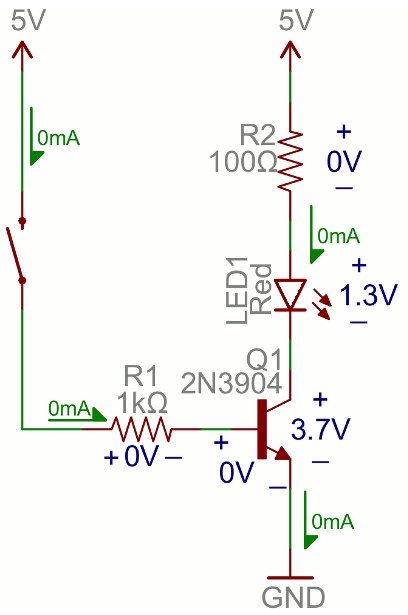
\includegraphics[width=150pt]{tran16}
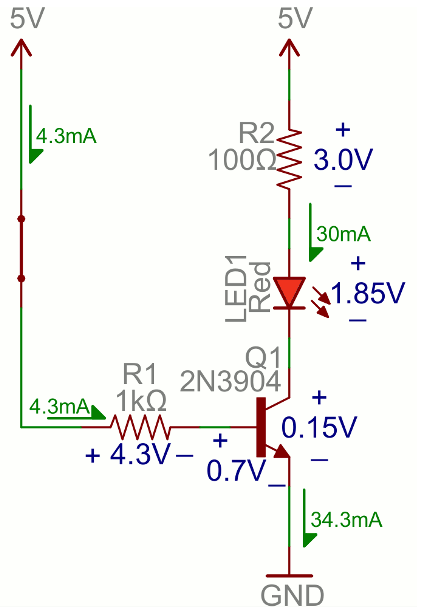
\includegraphics[width=150pt]{tran16b}
\end{center}

The resistor needs to be large enough to effectively limit the current, but small enough to feed the base enough current. 1mA to 10mA will usually be enough, but check your transistor's datasheet to make sure.

\subsection*{Digital Logic}

Transistors can be combined to create all our fundamental logic gates: AND, OR, and NOT.\\

(Note: These days MOSFETS are more likely to be used to create logic gates than BJTs. MOSFETs are more power-efficient, which makes them the better choice.)\\

\subsubsection*{Inverter}

Here’s a transistor circuit that implements an \textbf{inverter}, or NOT gate:

\begin{center}
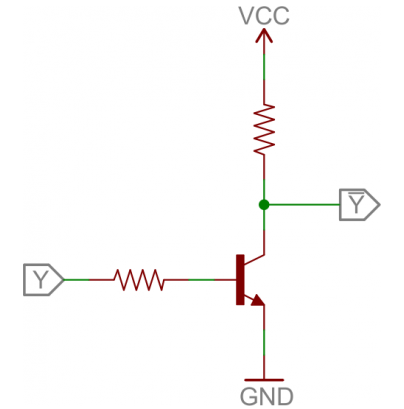
\includegraphics[width=150pt]{tran17}
\end{center}

Here a high voltage into the base will turn the transistor on, which will effectively connect the collector to the emitter. Since the emitter is connected directly to ground, the collector will be as well (though it will be slightly higher, somewhere around $V_{CE}(sat)$ $\approx$ (0.05-0.2V). If the input is low, on the other hand, the transistor looks like an open circuit, and the output is pulled up to $V_{CC}$.\\

(This is actually a fundamental transistor configuration called common emitter. More on that later.)\\

\subsubsection*{AND Gate}

Here are a pair of transistors used to create a 2-input AND gate:

\begin{center}
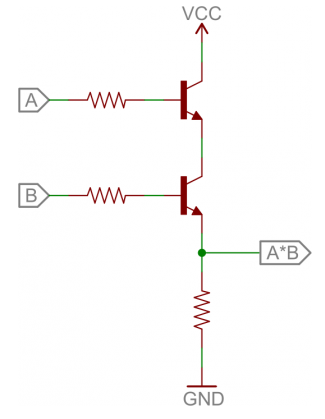
\includegraphics[width=150pt]{tran18}
\end{center}

If either transistor is turned off, then the output at the second transistor's collector will be pulled low. If both transistors are "on" (bases both high), then the output of the circuit is also high.

\subsubsection*{OR Gate}

And, finally, here is a 2-input OR gate:

\begin{center}
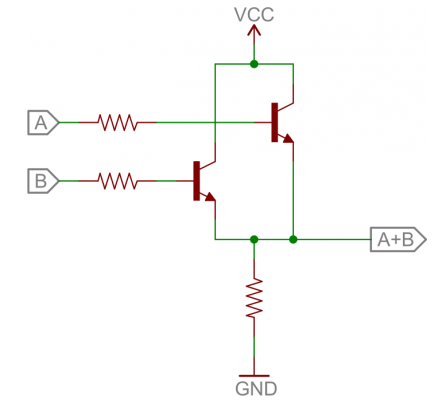
\includegraphics[width=150pt]{tran19}
\end{center}

In this circuit, if either (or both) A or B are high, that respective transistor will turn on, and pull the output high. If both transistors are off, then the output is pulled low through the resistor.

\subsection*{H-Bridge}

An H-bridge is a transistor-based circuit capable of driving motors both clockwise and counter-clockwise. It is an incredibly popular circuit - the driving force behind countless robots that must be able to move both forward and backward.\\

Fundamentally, an H-bridge is a combination of four transistors with two inputs lines and two outputs:

\begin{center}
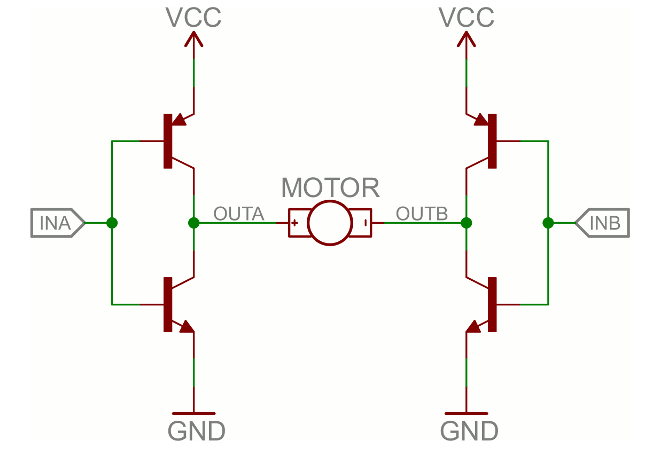
\includegraphics[width=300pt]{tran20a}
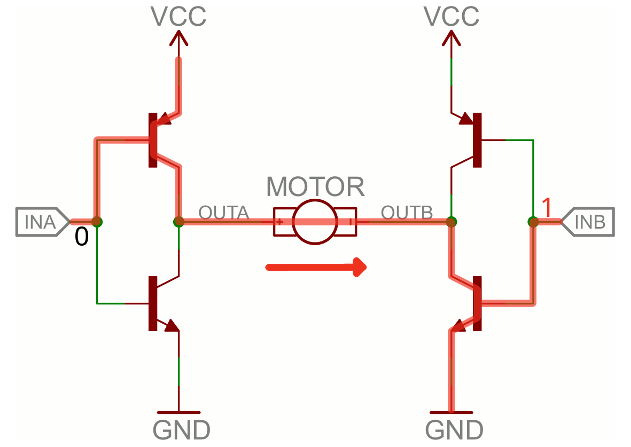
\includegraphics[width=170pt]{tran20b}
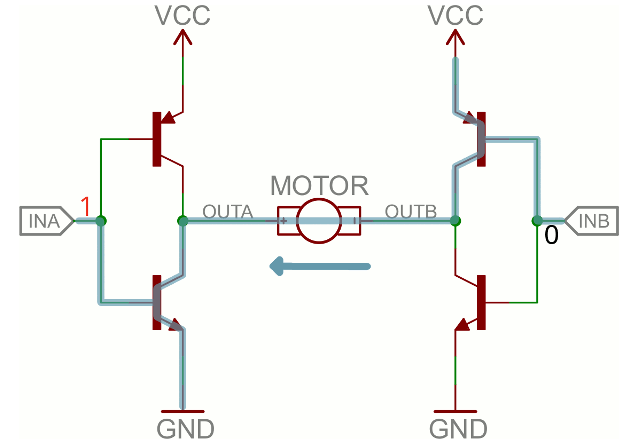
\includegraphics[width=170pt]{tran20c}
\end{center}

Note: there is usually quite a bit more to a well-designed H-bridge including flyback diodes, base resistors and Schmidt triggers.)\\

If both inputs are the same voltage, the outputs to the motor will be the same voltage, and the motor won't be able to spin. But if the two inputs are opposite, the motor will spin in one direction or the other.\\

The H-bridge has a truth table that looks a little like this:\\

\begin{center}
 \begin{tabular}{|c|c|c|c|c|}
\hline 
\textbf{Input A} & \textbf{Input B} & \textbf{Output A} & \textbf{Output B} & \textbf{Motor direction} \\ 
\hline 
0 & 0 & 1 & 1 & Stopped (branking) \\ 
\hline 
0 & 1 & 1 & 0 & Clockwise \\ 
\hline 
1 & 0 & 0 & 1 & Counter-clockwise \\ 
\hline 
1 & 1 & 0 & 0 & Stopped (branking) \\ 
\hline 
\end{tabular}
 \end{center} 

\subsection*{Oscillators}

An oscillator is a circuit that produces a periodic signal that swings between a high and low voltage. Oscillators are used in all sorts of circuits: from simply blinking an LED to the producing a clock signal to drive a microcontroller. There are lots of ways to create an oscillator circuit including quartz crystals, op amps, and, of course, transistors.\\

Here is an example oscillating circuit, which we call an astable multivibrator. By using feedback we can use a pair of transistors to create two complementing, oscillating signals.

\begin{center}
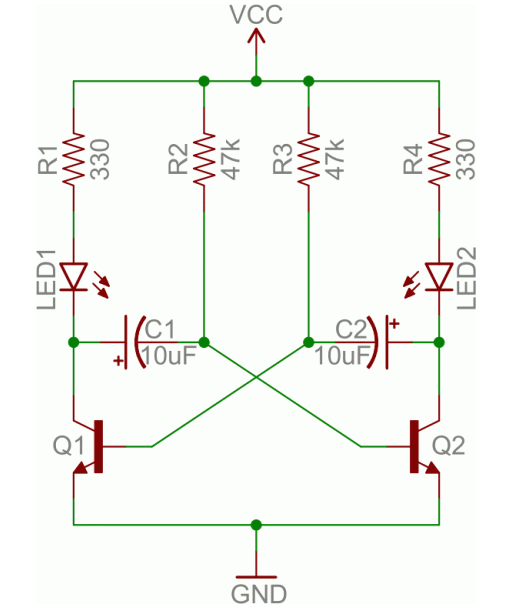
\includegraphics[width=200pt]{tran21}
\end{center}

Aside from the two transistors, the capacitors are the real key to this circuit. The caps alternatively charge and discharge, which causes the two transistors to alternatively turn on and off.\\

Analyzing this circuit's operation is an excellent study in the operation of both caps and transistors. To begin, assume $C1$ is fully charged (storing a voltage of about $V_{CC}$), $C2$ is discharged, $Q1$ is on, and $Q2$ is off. Here is what happens after that:

\begin{itemize}
\item If $Q1$ is on, then $C1's$ left plate (on the schematic) is connected to about 0V. This will allow $C1$ to discharge through $Q1's$ collector.
\item While $C1$ is discharging, $C2$ quickly charges through the lower value resistor - $R4$.
\item Once $C1$ fully discharges, its right plate will be pulled up to about 0.6V, which will turn on $Q2$.
\item At this point we have swapped states: $C1$ is discharged, $C2$ is charged, $Q1$ is off, and $Q2$ is on. Now we do the same dance the other way.
\item $Q2$ being on allows $C2$ to discharge through $Q2's$ collector.
\item While $Q1$ is off, $C1$ can charge, relatively quickly through $R1$.
\item Once $C2$ fully discharges, $Q1$ will be turn back on and we are back in the state we started in.
\end{itemize}

It can be hard to wrap your head around. You can find another excellent demo of this circuit here.\\

By picking specific values for $C1$, $C2$, $R2$, and $R3$ (and keeping $R1$ and $R4$ relatively low), we can set the speed of our multivibrator circuit:

$$f = \frac{1}{ln(2) (R2*C1 + R3*C2)}$$

So, with the values for caps and resistors set to $10\mu F$ and $47k\Omega$ respectively, our oscillator frequency is about $1.5 Hz$. That means each LED will blink about 1.5 times per second.\\

As you can probably already see, there are tons of circuits out there that make use of transistors. But we have barely scratched the surface. These examples mostly show how the transistor can be used in saturation and cutoff modes as a switch, but what about amplification? Time for more examples!


\section*{Applications II: Amplifiers}

Some of the most powerful transistor applications involve amplification: turning a low power signal into one of higher power. Amplifiers can increase the voltage of a signal, taking something from the $\mu V$ range and converting it to a more useful $mV$ or $V$ level. Or they can amplify current, useful for turning the $\mu A$ of current produced by a photodiode into a current of much higher magnitude. There are even amplifiers that take a current in, and produce a higher voltage, or viceversa (called transresistance and transconductance respectively).\\

Transistors are a key component to many amplifying circuits. There are a seemingly infinite variety of transistor amplifiers out there, but fortunately a lot of them are based on some of these more primitive circuits. Remember these circuits, and, hopefully, with a bit of pattern matching, you can make sense of more complex amplifiers.

\subsection*{Common Configurations}

Three of the most fundamental transistor amplifiers are: common emitter, common collector and common base. In each of the three configurations one of the three nodes is permanently tied to a common voltage (usually ground), and the other two nodes are either an input or output of the amplifier.

\subsubsection*{Common Emitter}

Common emitter is one of the more popular transistor arrangements. In this circuit the emitter is tied to a voltage common to both the base and emitter (usually ground). The base becomes the signal input, and the collector becomes the output.

\begin{center}
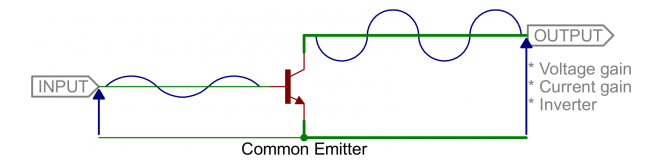
\includegraphics[width=400pt]{tran22}
\end{center}

The common emitter circuit is popular because it is well-suited for voltage amplification, especially at low frequencies. They are great for amplifying audio signals, for example. If you have a small $1.5V$ peak-to-peak input signal, you could amplify that to a much higher voltage using a slightly more complicated circuit, like:

\begin{center}
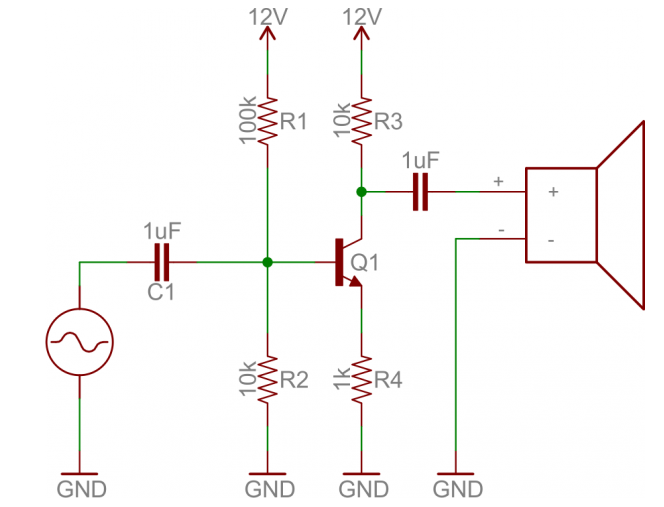
\includegraphics[width=300pt]{tran23}
\end{center}

One quirk of the common emitter, though, is that it inverts the input signal (compare it to the inverter from the last page!).

\subsubsection*{Common Collector (Emitter Follower)}

If we tie the collector pin to a common voltage, use the base as an input, and the emitter as an output, we have a common collector. This configuration is also known as an emitter follower.

\begin{center}
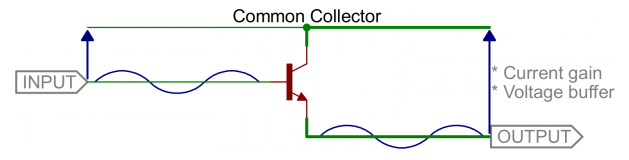
\includegraphics[width=400pt]{tran24}
\end{center}

The common collector doesn't do any voltage amplification (in fact, the voltage out will be 0.6V lower than the voltage in). For that reason, this circuit is sometimes called a voltage follower.\\

This circuit does have great potential as a current amplifier. In addition to that, the high current gain combined with near unity voltage gain makes this circuit a great voltage buffer. A voltage buffer prevents a load circuit from undesirably interfering with the circuit driving it.\\

For example, if you wanted to deliver 1V to a load, you could go the easy way and use a voltage divider, or you could use an emitter follower.\\

\begin{center}
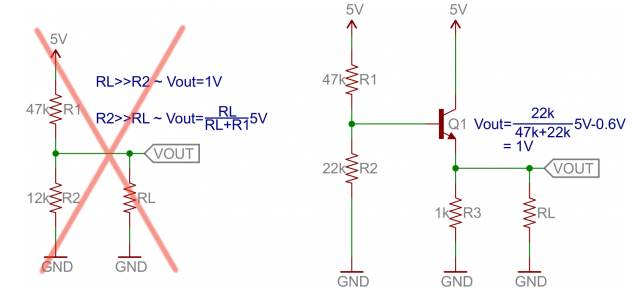
\includegraphics[width=400pt]{tran25}
\end{center}

As the load gets larger (which, conversely, means the resistance is lower) the output of the voltage divider circuit drops. But the voltage output of the emitter follower remains steady, regardless of what the load is. Bigger loads can’t “load down” an emitter follower, like they can circuits with larger output impedances.

\subsubsection*{Common Base}

We will talk about common base to provide some closure to this section, but this is the least popular of the three fundamental configurations. In a common base amplifier, the emitter is an input and the collector an output. The base is common to both.

\begin{center}
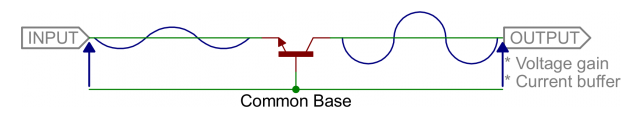
\includegraphics[width=400pt]{tran26}
\end{center}

Common base is like the anti-emitter-follower. It is a decent voltage amplifier, and current in is about equal to current out (actually current in is slightly greater than current out).\\

The common base circuit works best as a current buffer. It can take an input current at a low input impedance, and deliver nearly that same current to a higher impedance output.

\subsubsection*{In Summary}

These three amplifier configurations are at the heart of many more complicated transistor amplifiers. They each have applications where they shine, whether they are amplifying current, voltage, or buffering.

\begin{center}
\begin{tabular}{|c|c|c|c|}
\hline 
- & \textbf{Common emitter} & \textbf{Common collector} & \textbf{Common base} \\ 
\hline 
\textbf{Voltage gain} & Medium & Low & High \\ 
\hline 
\textbf{Current gain} & Medium & High & Low \\ 
\hline 
\textbf{Input impedance} & Medium & High & Low \\ 
\hline 
\textbf{Output impedance} & Medium & Low & High \\ 
\hline 
\end{tabular} 
\end{center}

\subsection*{Multistage Amplifiers}

We could go on and on about the great variety of transistor amplifiers out there. Here are a few quick examples to show off what happens when you combine the single-stage amplifiers above:

\subsubsection*{Darlington}

The Darlington amplifier runs one common collector into another to create a high current gain amplifier.

\begin{center}
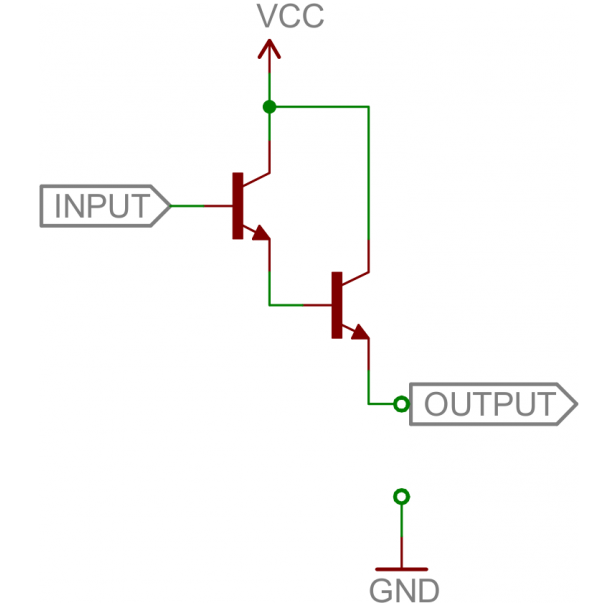
\includegraphics[width=250pt]{tran27}
\end{center}

Voltage out is about the same as voltage in (minus about $1.2V-1.4V$), but the current gain is the product of two transistor gains. That is $2\beta$, upwards of 1000.\\

The Darlington pair is a great tool if you need to drive a large load with a very small input current.

\subsubsection*{Differential Amplifier}

A differential amplifier subtracts two input signals and amplifies that difference. It is a critical part of feedback circuits, where the input is compared against the output, to produce a future output. Here is the foundation of the differential amp:

\begin{center}
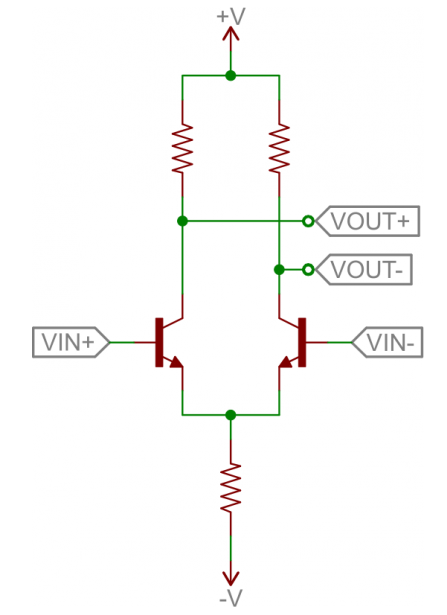
\includegraphics[width=200pt]{tran28}
\end{center}

This circuit is also called a long tailed pair. It is a pair of common-emitter circuits that are compared against each other to produce a differential output. Two inputs are applied to the bases of the transistors; the output is a differential voltage across the two collectors.

\subsubsection*{Push-Pull Amplifier}

A push-pull amplifier is a useful "final stage" in many multi-stage amplifiers. It is an energy efficient power amplifier, often used to drive loudspeakers.\\

The fundamental push-pull amp uses an NPN and PNP transistor, both configured as common collectors:

\begin{center}
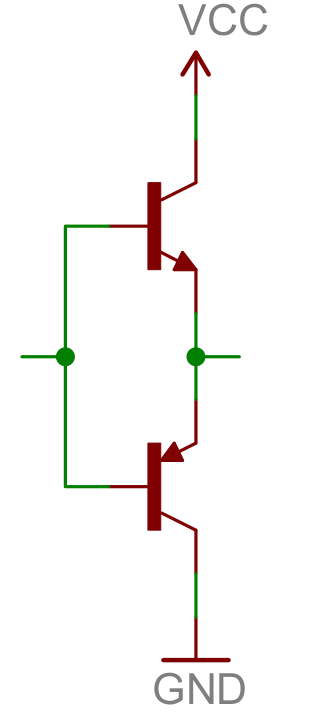
\includegraphics[width=100pt]{tran29}
\end{center}

The push-pull amp does not really amplify voltage (voltage out will be slightly less than that in), but it does amplify current. It is especially useful in bi-polar circuits (those with positive and negative supplies), because it can both "push" current into the load from the positive supply, and "pull" current out and sink it into the negative supply.\\

If you have a bi-polar supply (or even if you do not), the push-pull is a great final stage to an amplifier, acting as a buffer for the load.

\subsubsection*{Putting Them Together (An Operational Amplifier)}

Let's look at a classic example of a multi-stage transistor circuit: an Op Amp. Being able to recognize common transistor circuits, and understanding their purpose can get you a long way! Here is the circuit inside an LM3558, a really simple op amp:

\begin{center}
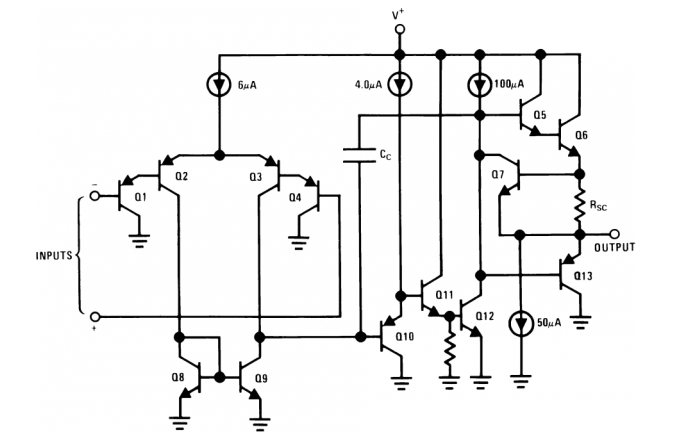
\includegraphics[width=380pt]{tran30}
\end{center}

There is certainly more complexity here than you may be prepared to digest, however you might see some familiar topologies:

\begin{itemize}
\item $Q1$, $Q2$, $Q3$, and $Q4$ form the input stage. Looks a lot like an common collector ($Q1$ and $Q4$) into a differential amplifier, right? It just looks upside down, because it is using PNP's. These transistors help to form the input differential stage of the amplifier.
\item $Q11$ and $Q12$ are part of the second stage. $Q11$ is a common collector and $Q12$ is a common emitter. This pair of transistors will buffer the signal from $Q3's$ collector, and provide a high gain as the signal goes to the final stage.
\item $Q6$ and $Q13$ are part of the final stage, and they should look familiar as well (especially if you ignore RSC) - it is a push-pull! This stage buffers the output, allowing it to drive larger loads.
\item There are a variety of other common configurations in there that we have not talked about. $Q8$ and $Q9$ are configured as a current mirror, which simply copies the amount of current through one transistor into the other.
\end{itemize}

After this crash course in transistors, we wouldn't expect you to understand what is going on in this circuit, but if you can begin to identify common transistor circuits you are on the right track!

\textbf{Note:} Images used were downloaded from \textbf{Sparkfun.com}.

\end{document}